\documentclass[aps,twocolumn,nobalancelastpage]{revtex4}

\input{preamble}

\begin{document}

\title{Exercise 1: Matrices and Linear Algebra}
\author{Drew Silcock}
\affiliation{Physics Department, University of Bristol}
\date{\today}

\maketitle

\section{Introduction}
\label{sec:introduction}

In this exercise three problems are solved. Firstly, a program is written to solve the Laplace equation in two dimensions using the method of finite difference. This is then applied to the parallel plate capacitor and compared to the idealised infinite plate parallel plate capacitor and its properties. Finally, the heat diffusion equation is solved for an iron rod using the implicit finite difference method, and by solving a set of linear equations to iterate forwards in time.
\section{Relaxation Methods}
\label{sec:relaxation_methods}

A common method of solving partial differential equations, both linear and nonlinear, is by iterative relaxation methods. Here this means taking advantage of the finite difference discretisation of the differential equation. The essential method is to use a given iteration equation, called the finite difference equation, to repeatedly iterate all nodes until a particular convergence criterion is satisfied. The grid of nodes is initially set as random guesses, and any boundary conditions must be reimposed on each iteration.

\subsection{Laplace Equation}
There are two main application of the finite difference method here. The first is to the Poisson equation,
\begin{equation}
    \nabla^2 \varphi = -\rho,
    \label{eqn:poisson}
\end{equation} in the specific case where $\rho = 0$, i.e. this becomes the Laplace equation. This produces the following finite difference iteration equation:
\begin{align}
    \varphi(x_i,y_i) = \frac{1}{4}\bigg[&\varphi(x_{i-1},y_j)+\varphi(x_{i+1},y_j)+ \notag \\
        & \varphi(x_i,y_{i-1})+\varphi(x_i,y_{i+1})+ \label{eqn:iteration} \\
        & \rho(x_i,y_j)h^2\bigg] \notag
\end{align}
where $x_i,y_j$ are points on the grid and $\rho = 0$, i.e. there are no sources. In this case then this iteration simply becomes the average value of the nearest neighbour points on the grid.

There are two methods of solving this equation.

\subsubsection{Jacobi Method}

There are at any time two distinct grids of nodes. When the finite difference equation is used to iterate a node, producing the new value, this value is stored in the new grid so that all iterations are acted upon by the old grid and produce values which go into the new grid. This means that all iterations are based entirely on the values from the original grid.

\subsubsection{Gauss-Seidel Method}

Another possible iteration method is known as the Gauss-Seidel method. In this method, the value produced by iterating at a node using the same finite difference equation is stored in the original grid. This means that all iterations are based partly on values from the original grid and partly on new values obtained from already completed iterations.

\subsection{Heat Diffusion Equation}

The second main application of the finite difference method here is to solving the heat diffusion equation. There are two primary finite difference iteration methods for the solving the heat diffusion equation:

\subsubsection{Explicit Forward Difference Method}
The explicit forward difference (also known as the Forward Time, Centred Space method or FTCS method) uses the following iteration equation to go from time $t$ to time $t+\delta t$:
\begin{align}
    \frac{\phi(x_i,t+\delta t)}{\delta t} = \frac{\alpha}{h^2}\big[&\phi(x_{i-1},t) + \phi(x_{i+1},t) \notag \\
                                                               & - 2\phi(x_i,t)\big].\label{eqn:explicit}
\end{align}
This equation is unstable for $\frac{\alpha \delta t}{h^2} \leq \frac{1}{2}$ (where $\delta t$ is the time step and $h$ is the distance between nodes in the discretised rod). For the iron rod, $\alpha = \SI{23}{\milli\meter\per\second}$, so taking a reasonable grid spacing of $h = \SI{1}{\centi\metre}$ and time step of $\delta t = \SI{10}{\second}$ results in Equation \ref{eqn:explicit} becoming unstable and unusable. The second, generally more numerically intensive implicit finite difference method is therefore resorted to.

\subsubsection{Implicit Backward Difference Method}
The implicit forward difference (also known as the Backward Time, Centred Space method or BTCS method) uses the following subtly different iteration equation to go from time $t+\delta t$ to time $t$:
\begin{align}
    \frac{\phi(x_i,t+\delta t) - \phi(x_i,t)}{\delta t} = \frac{\alpha}{h^2}\big[&\phi(x_{i-1},t+\delta t) \notag \\
                                                                                 & + \phi(x_{i+1},t+\delta t) \label{eqn:implicit} \\
                                                                                 & - 2\phi(x_i,t+\delta t)\big]. \notag
\end{align}
This iteration method converges for all values of $\frac{\alpha \delta t}{h^2}$, and is thus used for the final part of this exercise. It does, however, require solving a linear set of equations, which can be arranged as a matrix equation and solved by inverting the matrix of prefactors, $\text{P}$, as in $\text{P}\bm{\phi}(t+\delta t) = \bm{\phi}(t) \implies \bm{\phi}(t+\delta t) = \bm{\phi}(t) \text{P}^{-1}$, where $\bm{\phi}(t)$ runs over all nodes in the discretised rod at time $t$.
\section{Solving Laplace's Equation in Two Dimensions}
\label{sec:laplace}

Here Laplace's equation in two dimensions,
\begin{equation}
    \nabla^2 \varphi = 0,
\end{equation}
is solved using the finite difference equation given in Equation \ref{eqn:iteration} with $\rho = 0$. The chosen convergence condition is that the maximum change in any node is less than an absolute error tolerance, called $\epsilon$. By default $\epsilon$ is set to $10^{-5}$, but choosing a different scale for the charge density requires altering this to be appropriate, e.g. if the charges involved are $\mathcal{O}(10^{-6})$, the absolute error tolerance should be $\sim 10^{-11}$.\todo{I might change this.} All non-boundary nodes were set to random guesses between 0 and 1. The number of iterations was capped at \texttt{max\_it}$=10000$.

\subsection{Basic Verification}
\label{subsec:basic_verification}

The program has in-built boundary conditions for a parallel plate capacitor, a plane equipotential, a single point charge-like equipotential in the middle of the grid, a net with constant potential around the edges of the grid and a cross equipotential. The resulting solutions are plotted in Figures \ref{fig:basic_examples}.

\begin{figure}
    \centering
    \subfloat[Contour plot]{
        \includegraphics[width=0.3\linewidth]{graphs/examples/plane_contour.eps}
        \label{subfig:plane_cont}
    }
    \subfloat[Surface plot]{
        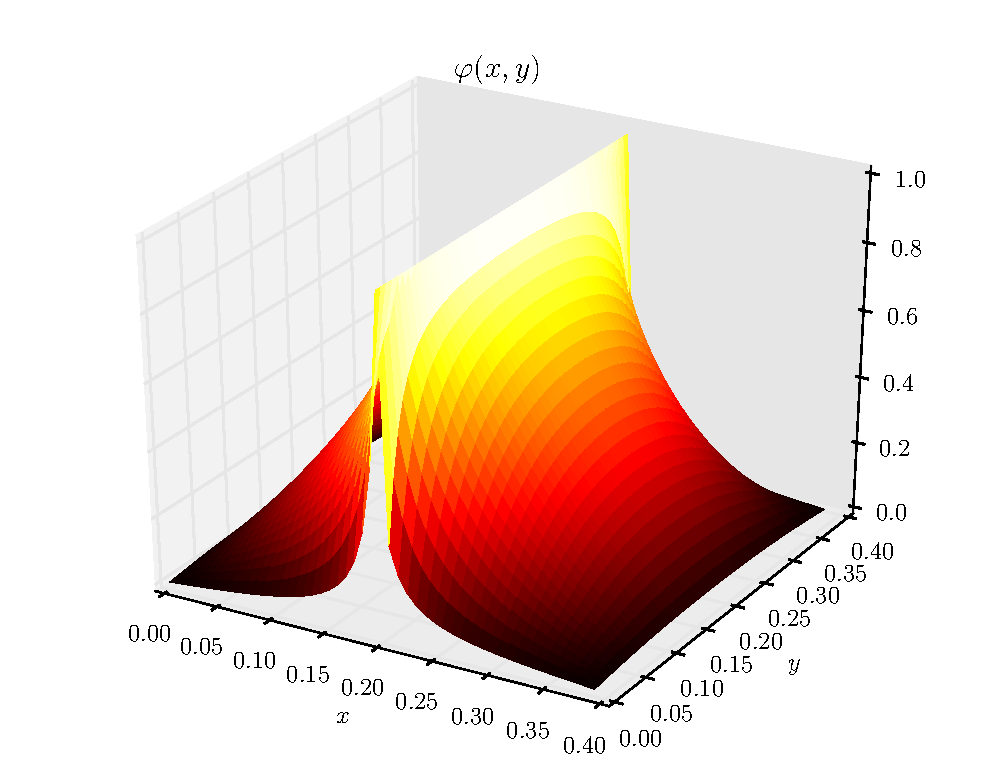
\includegraphics[width=0.3\linewidth]{graphs/examples/plane_surf.eps}
        \label{subfig:plane_surf}
    }
    \subfloat[Vector \textbf{E} field plot]{
        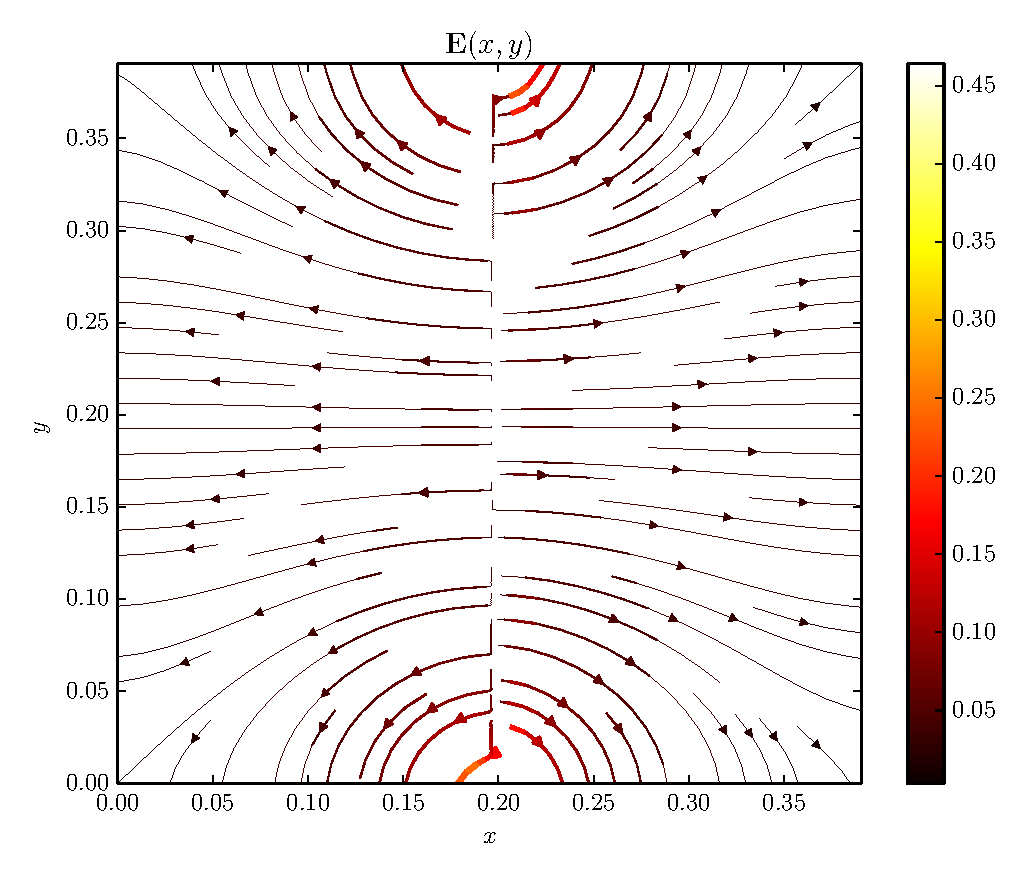
\includegraphics[width=0.3\linewidth]{graphs/examples/plane_vector.eps}
        \label{subfig:plane_vect}
    }
    \caption{Plots of the solution to the Laplace equation with boundary conditions of an equipotential plane.}
    \label{fig:plane}
\end{figure}

\begin{figure}
    \centering
    \subfloat[Contour plot]{
        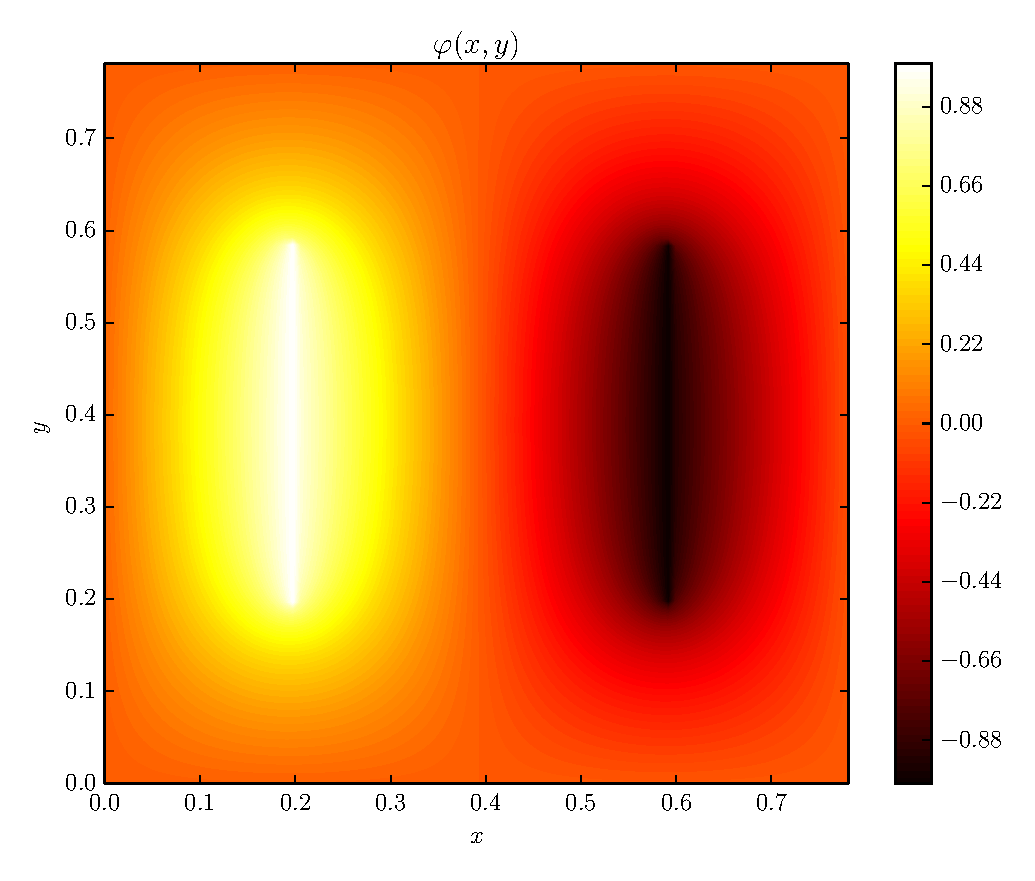
\includegraphics[width=0.3\linewidth]{graphs/examples/capacitor_contour.eps}
        \label{subfig:capacitor_cont}
    }
    \subfloat[Surface plot]{
        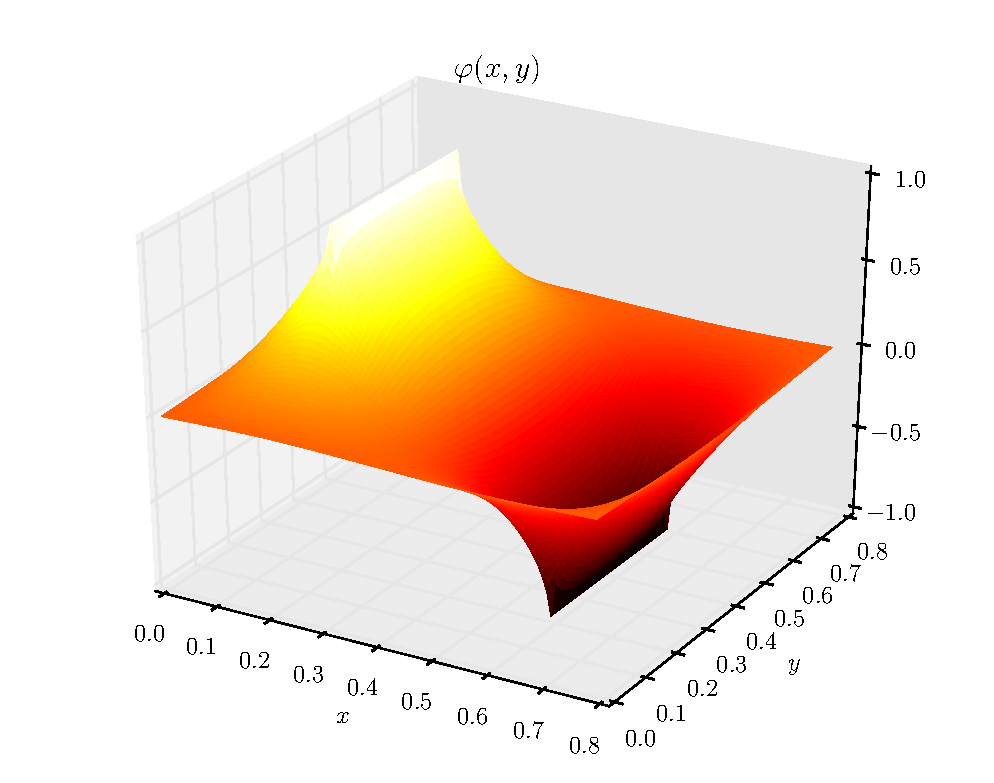
\includegraphics[width=0.3\linewidth]{graphs/examples/capacitor_surf.eps}
        \label{subfig:capacitor_surf}
    }
    \subfloat[Vector \textbf{E} field plot]{
        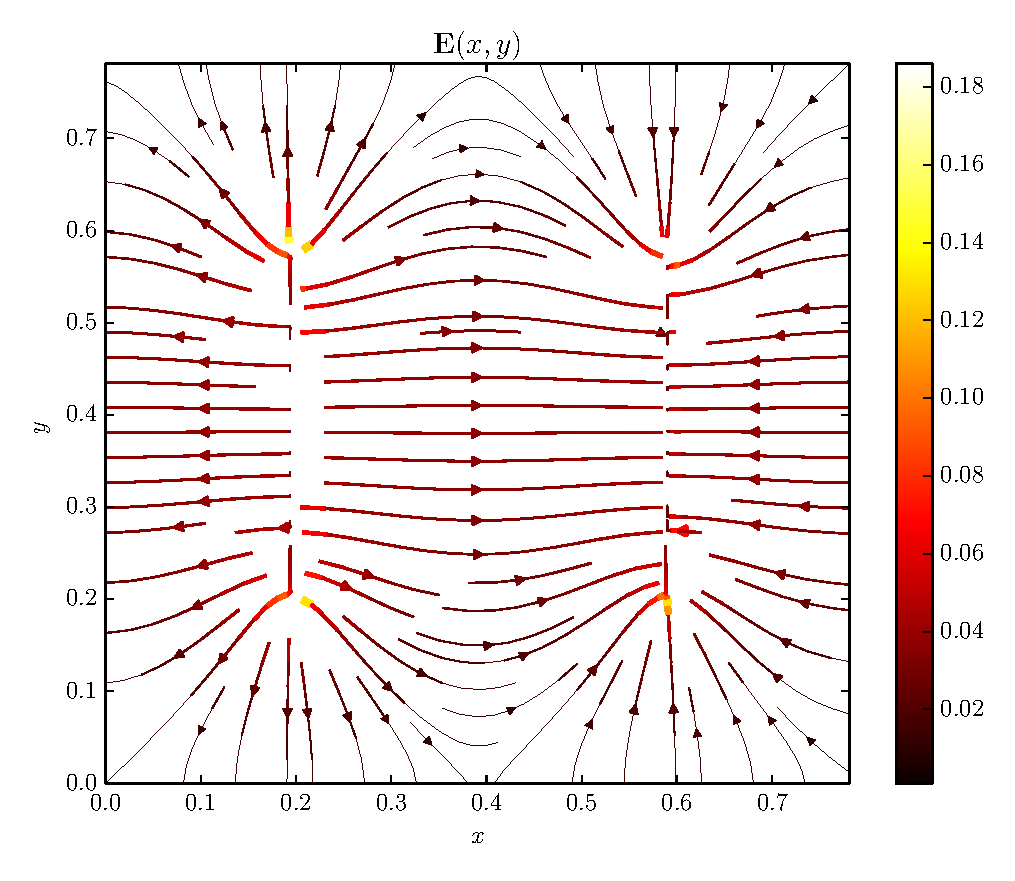
\includegraphics[width=0.3\linewidth]{graphs/examples/capacitor_vector.eps}
        \label{subfig:capacitor_vect}
    }
    \caption{Plots of the solution to the Laplace equation for a parallel plate capacitor.}
    \label{fig:plane}
\end{figure}

\begin{figure}
    \centering
    \subfloat[Contour plot]{
        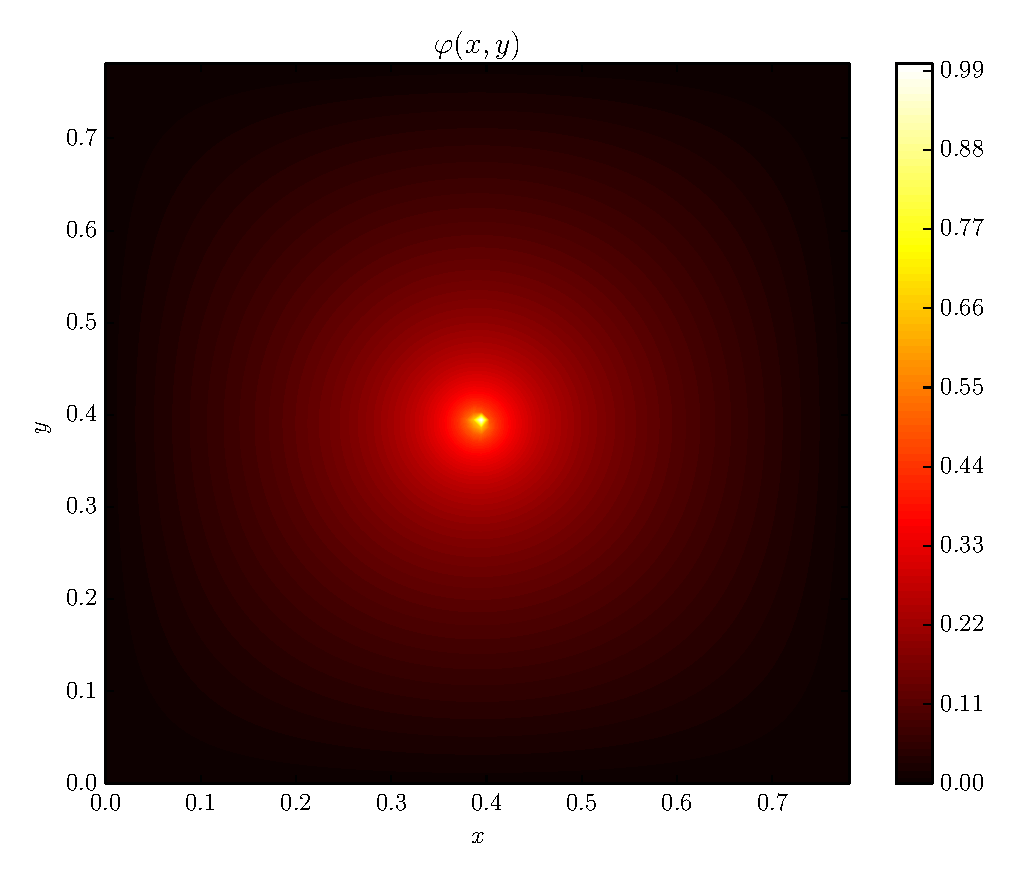
\includegraphics[width=0.3\linewidth]{graphs/examples/point_charge_contour.eps}
        \label{subfig:point_charge_cont}
    }
    \subfloat[Surface plot]{
        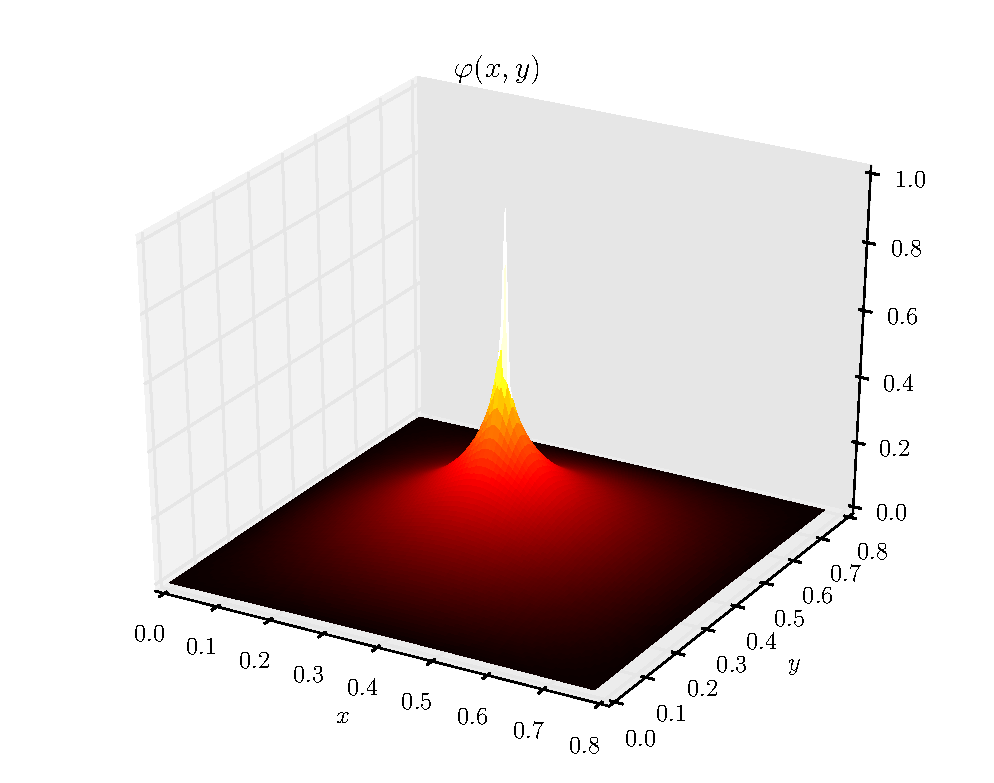
\includegraphics[width=0.3\linewidth]{graphs/examples/point_charge_surf.eps}
        \label{subfig:point_charge_surf}
    }
    \subfloat[Vector \textbf{E} field plot]{
        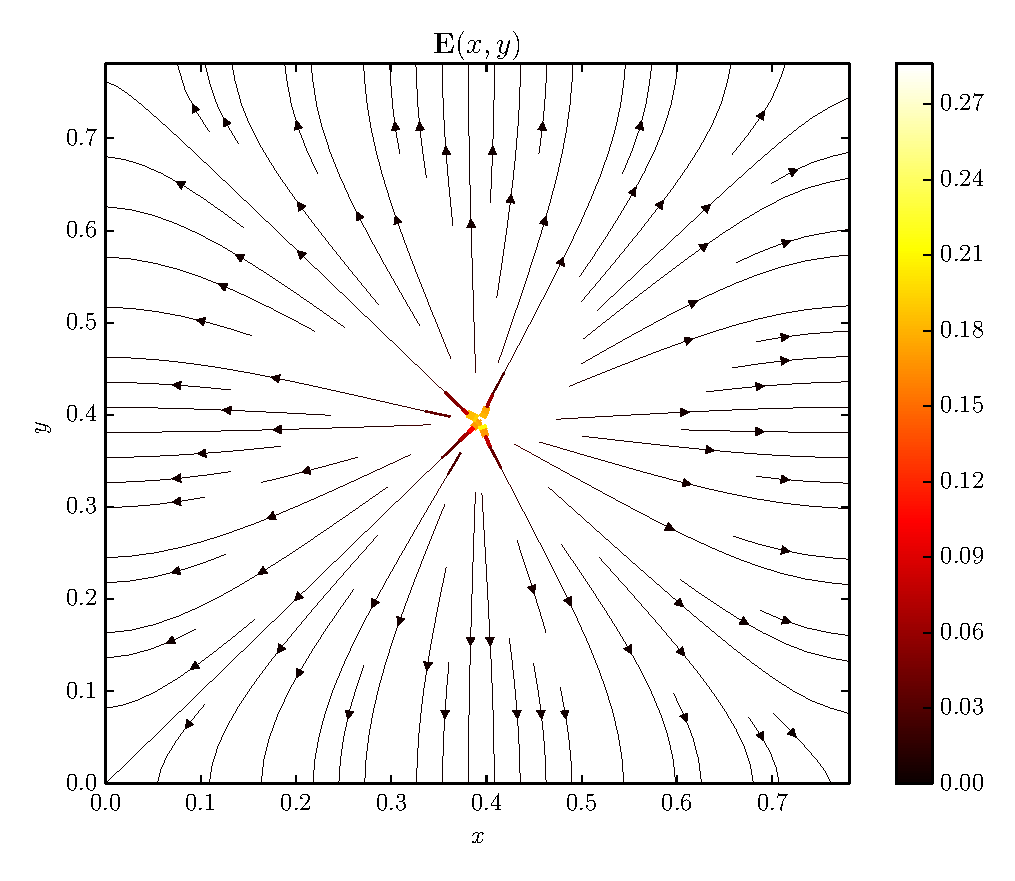
\includegraphics[width=0.3\linewidth]{graphs/examples/point_charge_vector.eps}
        \label{subfig:point_charge_vect}
    }
    \caption{Plots of the solution to the Laplace equation for a single constant potential point.}
    \label{fig:plane}
\end{figure}

\begin{figure}
    \centering
    \subfloat[Contour plot]{
        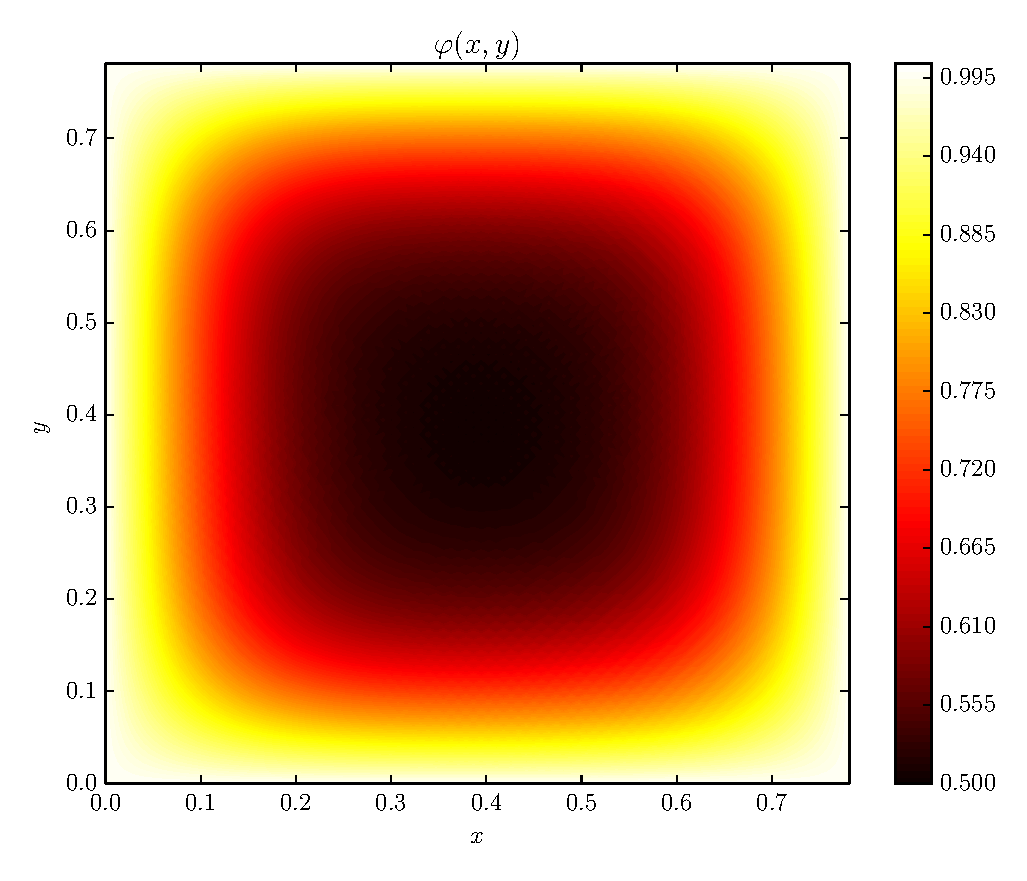
\includegraphics[width=0.3\linewidth]{graphs/examples/net_contour.eps}
        \label{subfig:net_cont}
    }
    \subfloat[Surface plot]{
        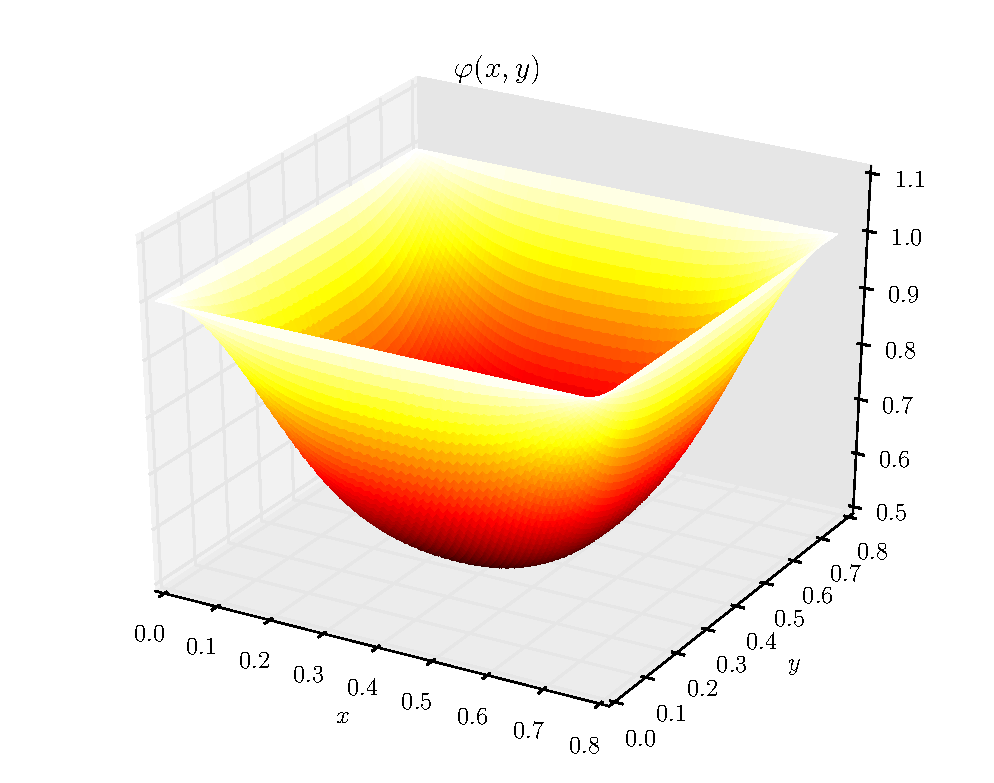
\includegraphics[width=0.3\linewidth]{graphs/examples/net_surf.eps}
        \label{subfig:net_surf}
    }
    \subfloat[Vector \textbf{E} field plot]{
        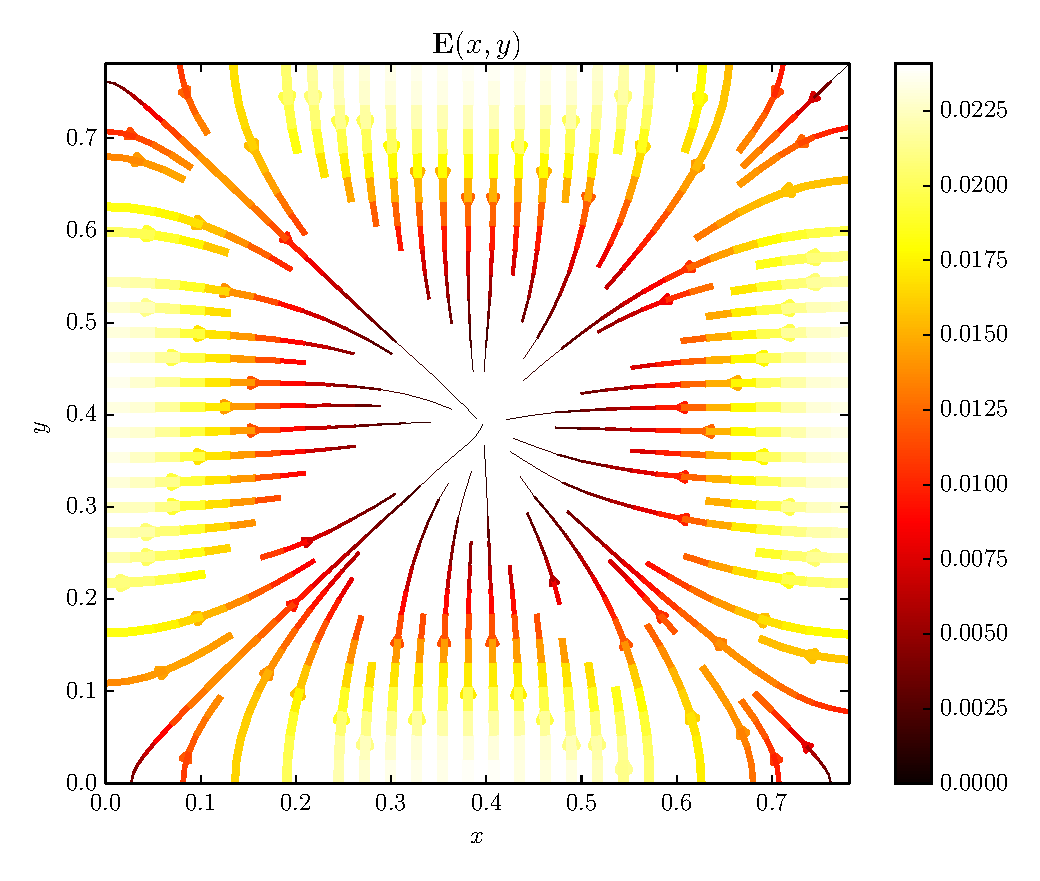
\includegraphics[width=0.3\linewidth]{graphs/examples/net_vector.eps}
        \label{subfig:net_vect}
    }
    \caption{Solution to the Laplace equation with edges of the grid held at constant positive potential.}
    \label{fig:plane}
\end{figure}

\begin{figure}
    \centering
    \subfloat[Contour plot]{
        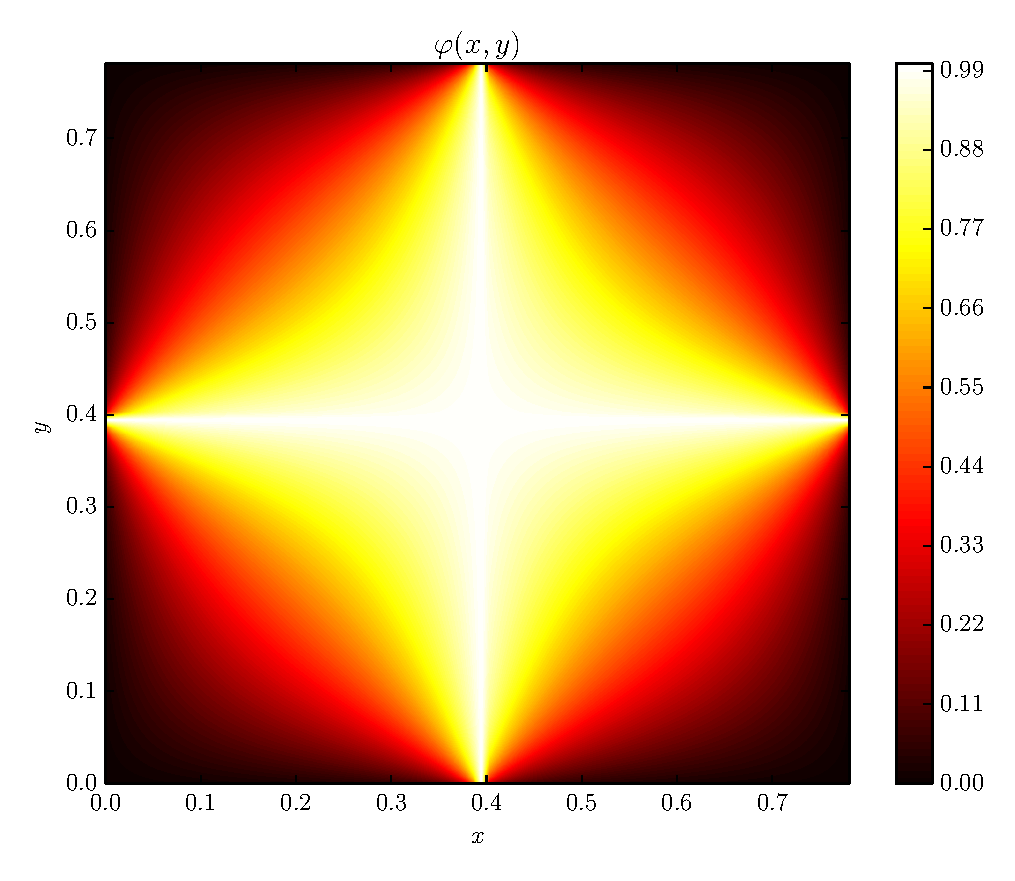
\includegraphics[width=0.3\linewidth]{graphs/examples/cross_contour.eps}
        \label{subfig:cross_cont}
    }
    \subfloat[Surface plot]{
        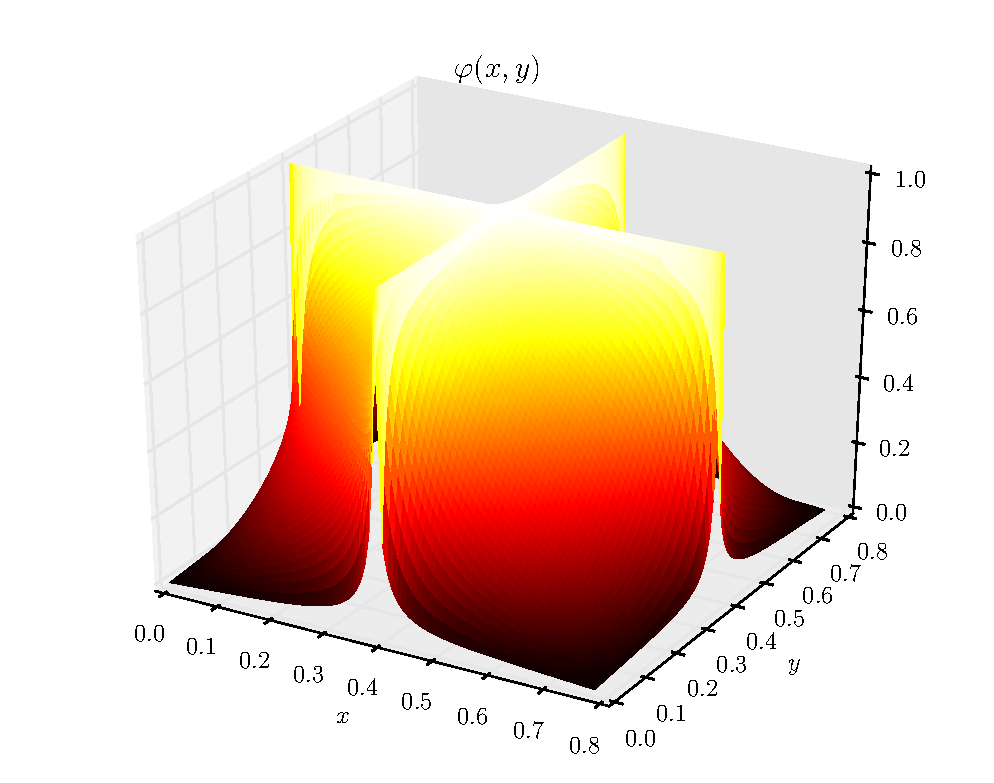
\includegraphics[width=0.3\linewidth]{graphs/examples/cross_surf.eps}
        \label{subfig:cross_surf}
    }
    \subfloat[Vector \textbf{E} field plot]{
        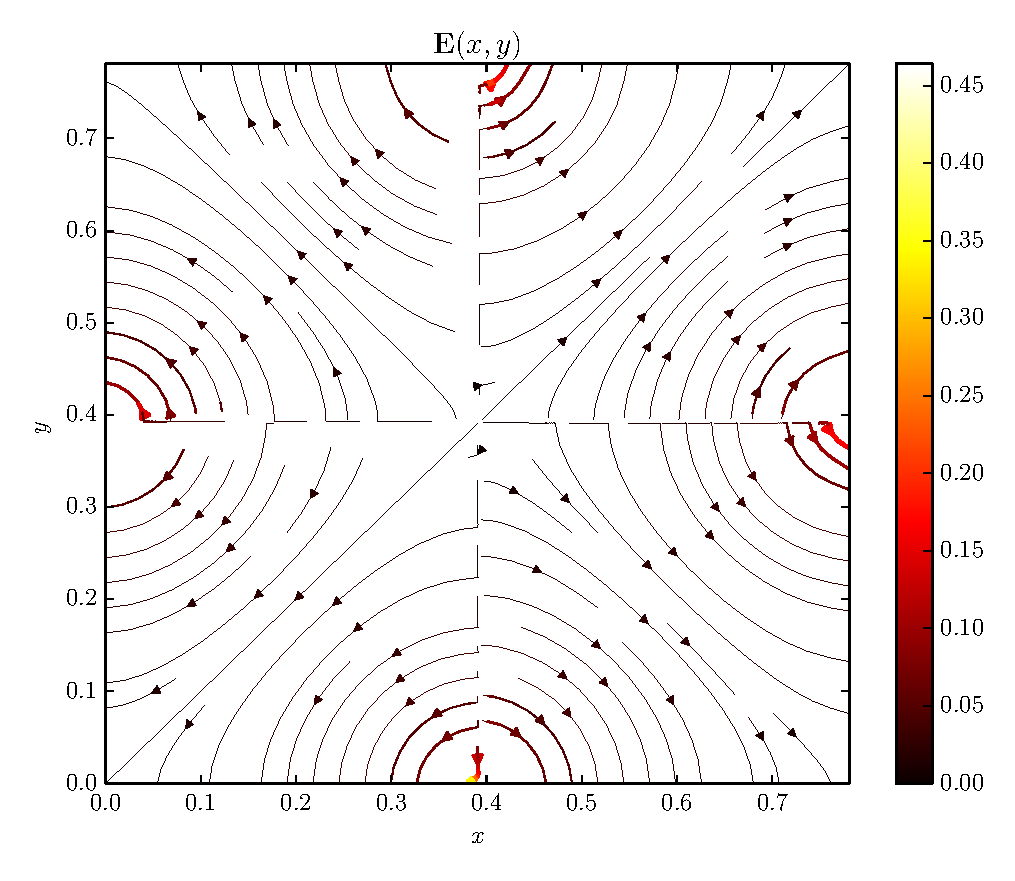
\includegraphics[width=0.3\linewidth]{graphs/examples/cross_vector.eps}
        \label{subfig:cross_vect}
    }
    \caption{Solution to the Laplace equation with equipotential cross overlaid on grid.}
    \label{fig:plane}
\end{figure}

\subsection{Convergence Condition}
\label{subsec:convergence_condition}

An absolute convergence condition is implemented to decide when the program has successfully iterated to the solution of the Laplace equation with the set boundary conditions. As compared to a relative convergence conditions, e.g. that no value changes by more than $X\%$, this has the disadvantage of depending on the boundary conditions applied to the system. So an absolute error tolerance of $\epsilon = \SI{0.01}{V}$ may be appropriate if the highest boundary condition is $\mathcal{O}(100)\si{V}$, but inappropriate if the potential boundary condition is $\mathcal{O}(0.1)$\si{V}. This is compensated for by the ability to manually change the error tolerance with the \texttt{--error} flag. By default this value is set at $10^{-4}$. When the boundary conditions are a single constant potential of \SI{1}{V} at the centre of the grid, the effect of a relatively large tolerance is to fatten the potential field around the point in the centre, as shown in Figure \ref{fig:tolerances}. This is because a too high $\epsilon$ means the iterations stop before a true solution is found. As there are no charges involved, the effect of each iteration is merely to average from the surrounding nodes. Hence when the program finishes the iterations early, it means it has prematurely ceased this averaging process and thus is higher near the central peak than it should physically be. \todo{Analysis of how changing the convergence condition changes the results out at the end, maybe with particular reference to the point charge which looks a bit squiffy for large tolerance.}

\begin{figure}
    \centering
    \subfloat[$\epsilon = 10^{-2}$]{
        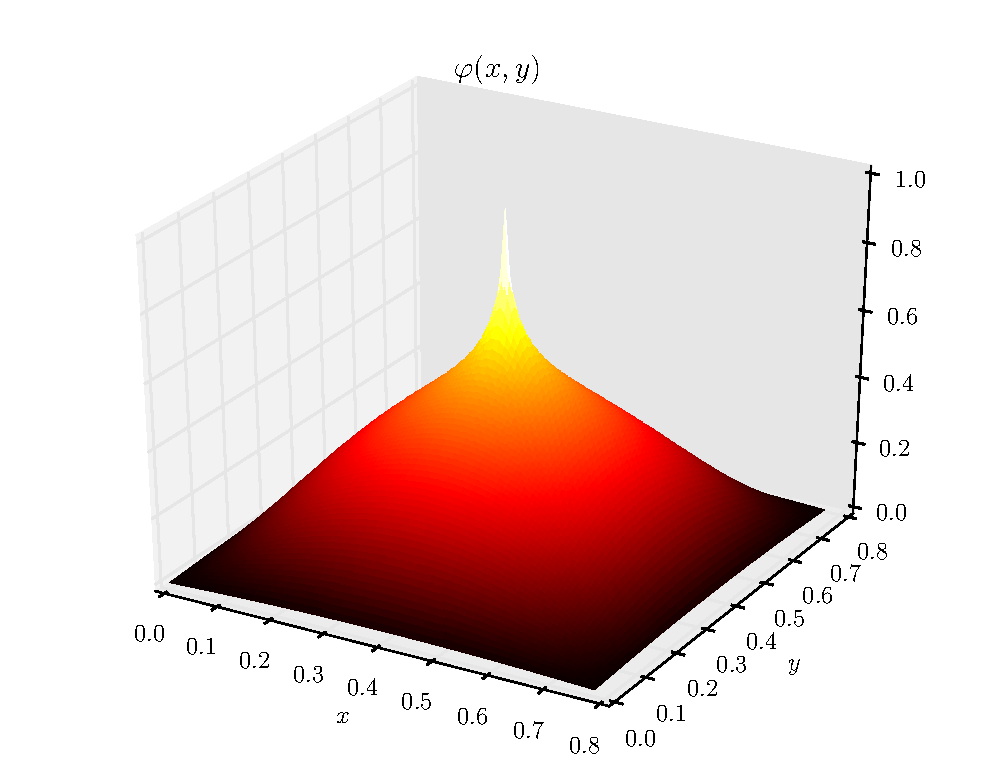
\includegraphics[width=0.5\linewidth]{graphs/tolerance/point_charge_error_1e-2_surf.eps}
        \label{subfig:error_1e-2}
    }
    \subfloat[$\epsilon = 10^{-6}$]{
        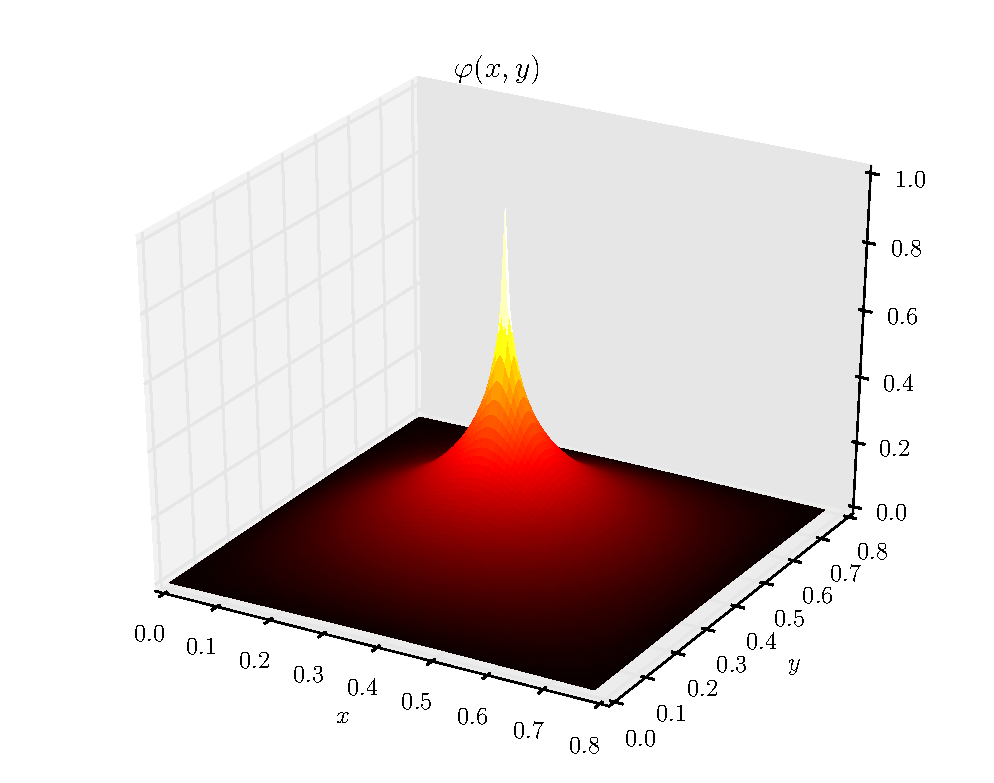
\includegraphics[width=0.5\linewidth]{graphs/tolerance/point_charge_error_1e-6_surf.eps}
        \label{subfig:error_1e-6}
    }
    \caption{Comparison of the effect of altering the absolute error tolerance, $\epsilon$, in the convergence condition on the resulting solution.}
    \label{fig:tolerances}
\end{figure}

\subsection{Iteration Method}
\label{subsec:convergence_condition}

Both the Jacobi and Gauss-Seidel iteration methods are implemented, with the option of which to use left up to the user with the positional argument \texttt{method} determining which to use. It is noticed that the Gauss-Seidel method is significantly faster than the Jacobi, particularly when computing the solution at high grid densities.\todo{A quantitative analysis of the difference in the timing between the two methods, including varying the grid density, with the aim of showing how much faster the Gauss-Seidel implementation is.}\todo{Comparison of consistency of results; include why it doesn't work for the net.}

\subsection{Grid Density}
\label{subsec:grid_density}

The default parameters of the grid density are a 50 by 50 grid. Changing the density significantly affects the time taken to find a converging solution. For the Jacobi method, the time taken to find the solution to the Laplace equation with the boundary conditions of a parallel plate capacitor...\todo{Detailed time analysis, possibly with table.} Combining high density with very low tolerance results in extremely long convergence times, as shown by \todo{Detailed analysis of what happens when you've got both high grid density (100x100) and low tolerance (1e-6).}.

\subsection{Grid Edges}
\label{subsec:grid_edges}


\section{Calculating Potential and Electric Field of Parallel Plate Capacitor}
\label{sec:parallel_plate_capacitor}
\section{Solving the Diffusion Equation for Iron Poker}
\label{sec:diffusion_equation}

\begin{thebibliography}{99}

    \bibitem{edwards2004}
        Ron Edwards, Bruce H. Falvo and David C. Larson,
        \emph{Elementary Linear Algebra (5th edition)},
        Chapter 10: Numerical Methods,
        Page 578.
        Houghton Mifflin Company,
        2004.

    \bibitem{golub1996}
        Gene H. Golub and Charles F. Van Loan,
        \emph{Matrix Computations (3rd edition)}.
        Johns Hopkins University Press,
        1996.

    \bibitem{demmel1997}
        James W. Demmel
        \emph{Applied Numerical Linear Algebra},
        Chapter 6: Iterative Methods for Linear Systems,
        Page 290.
        Society for Pure and Applied Mathematics,
        1997.

\end{thebibliography}

\end{document}